\chapter{Результаты проектирования}

\begin{annotation}
	В данной главе разрабатываются функциональные требования к разрабатываемой системе.
	Проектируется интерфейс модуля. Проектируется структура когнитивной карты.
	Проводится выбор инструментальных средств разработки.
\end{annotation}


\section{Разработка функциональных требований к системе}

Так как разрабатываемый модуль предназначен для решения задачи, которая
требует интенсивные вычисления, система должна быть реализована
с возможностью оптимизации данных вычислений. Распараллеливать вычисления
можно с помощью видеокарт. Это можно сделать с использованием фреймворка $ pytorch $.

Для проверки качества кода и его работоспособности, должны быть написаны тесты.
Автотесты помогают быстрее находить ошибки и регрессии в функциональности программы.

Эксперт должен иметь возможность задать произвольные концепты, описать
взаимосвязь между концептами явно или неявно, с помощью обученной карты.
Для того, чтобы обучить карту, эксперт должен иметь возможность загрузить
в нее исторические данные.

Эксперт должен иметь возможность построить графики зависимостей концептов
как по историческим данным, так и по предсказанным данным.

Таким образом, функциональные требования:
\begin{itemize}
	\item Возможность распараллеливания вычислений, с использованием фреймворка $pytorch$.
	\item Система непрерывной интеграции и автоматизированное тестирование.
	\item Поддержка заданных экспертом зависимостей между концептами.
	\item Поддержка зависимостей между концептами, вычисляемых с помощью LSTM.
	\item Модуль должен быть расширяемым. Нужна возможность определить пользовательскую функцию для постобработки данных, сгенерированных картой.
	\item Возможность динамических предсказаний. Динамические предсказания --- это
	предсказание, построенное на данных, которые были сгенерированы моделью на предыдущих шагах цикла.
	\item Возможность задать экзогенные параметры через карту.
\end{itemize}

% todo как идея, можно прикрутить мониторинг того, как обучается модель

\section{Архитектура системы непрерывной интеграции}

При отправке новых изменений в исходных текстах модуля,
удаленный репозиторий запускает обработчик тестов.
В этом обработчике запускаются команды, которые
проверяют работоспособность и качество кода в проекте.
В случае ошибок, pull-request блокируется, новые изменения не могут попасть
в ветку $ master $. На почту разработчика приходит уведомление, что
тесты не прошли. Процесс непрерывной интеграции представлен на диаграмме последовательности \ref{img:ci_sequence}.

\def\figurename{Рис}
\begin{figure}[t]
	\centering
	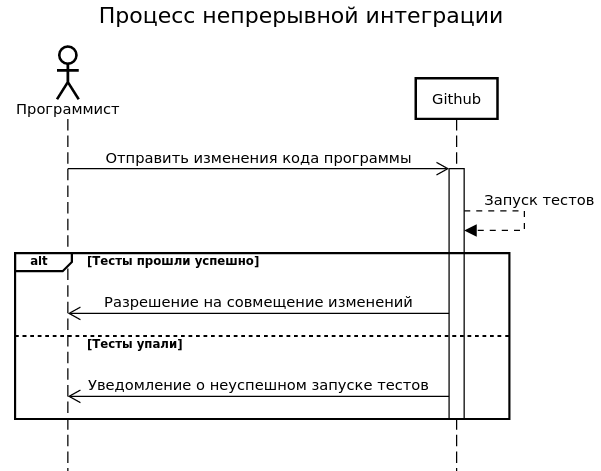
\includegraphics[height=7cm]{./img/ci_sequence.png}
	\caption{Диаграмма  последовательности процесса непрерывной интеграции}
	\label{img:ci_sequence}
\end{figure}

Когда тестов становится слишком много, для того, чтобы было
проще ориентироваться, где именно произошла ошибка,
можно пользоваться отдельными приложениями для построения
отчетов о тестировании. К таким отчетам можно прикреплять
дополнительную отладочную информацию, какую пожелает разработчик тестов.
Однако на данном этапе тестов не будет очень много и это пока что не целесообразно.

\section{Проектирование интерфейса модуля}

Для проектирования используется методология ООАП (объектно-ориентированный анализ и проектирование) \cite{маклафлин2013объектно}.

Работа с модулем должна состоять из следующих шагов:
\begin{itemize}
	\item Эксперт описывает карту и загружает в нее исходные данные.
	\item Карта обучается.
	\item Выполняется предсказание.
	\item Эксперт оценивает результат работы модели.
	\item На основании результатов карта модифицируется, дополняется.
\end{itemize}

\textbf{Описание концептов.}
При описании карты разработчик может задать
любое количество концептов и связать их любым образом.
Для моделирования будущих значений концепта
будет использоваться LSTM. Для того, чтобы обучить
эту модель предсказывать будущие значения данного концепта
нужны исторические данные. Это необходимый параметр для определения
нового концепта.
Также должна быть возможность задать произвольную модель,
которую эксперт может задать самостоятельно.

\textbf{Обучение.}
Теоретически, этот этап может быть распараллелен
за счет того, что исторические данные каждого концепта не меняются
и обучение каждого отдельного концепта происходит независимо.
Все модели, поддерживаемые картой должны
иметь общий интерфейс для обучения и вычисления,
чтобы не нарушать инкапсуляцию.
Метод обучения заданной экспертом модели должен быть скрыт внутри модели.

\textbf{Вычисление карты.}
Во время вычисления карты должны быть определены приоритеты
вычислений тех или иных концептов.
В зависимости от типа модели должна быть возможность получить
график функции потерь для модели, чтобы оценить качество предсказаний.

\textbf{Модификация карты.}
При добавлении новых концептов, нужно заново обучить
связанные концепты. При удалении концептов, потребуется
переобучение зависимых от удаленного концепта вершин.

\textbf{Моделирование с помощью когнитивной карты.}
Суть моделирования заключается не только в том, чтобы подобрать
оптимальные параметры для выборке для обучения и провалидировать обученную модель.
Эксперт может выдвинуть гипотезу, подстроить параметры модели
и исследовать, как будет вести себя система, анализировать
остатки, которые дает модель. Добавлять или удалять концепты с
целью найти объяснение тем или иным процессам. Так же эксперт
может добавлять в модель экзогенные параметры, которые могут
спрогнозировать поведение системы. Экзогенные параметры
должны быть определены экспертом не только на выборке для обучения,
но и на тестовой выборке. Предполагается, что эти параметры можно вычислить заранее.
В итоге эксперт должен получить граф, который описывает
исследуемый процесс. Этот граф можно интерпретировать
в соответствии с названиями каждой вершины, концепта.
Каждый концепт имеет свою историю значений. И может зависеть или
влиять на другие концепты. Таким образом, он отражает знания
эксперта об исследуемой системе. И с помощью функций, преобразований,
которые эксперт задал на этом графе, может быть получено предсказание
определенных значений концептов.

\textbf{Повторное обучение.}
Так же как и для модификации карты. Не обязательно переобучать всю карту целиком.
Если в этом есть необходимость, можно переобучить только часть карты.

Диаграмма классов спроектированного модуля представлена не рисунке \ref{img:class_diag}.
Классы моделей, которы могут быть использованы в качестве модели для вычисления
концептов, должны имплементировать 3 метода:
\begin{itemize}
	\item \verb|fit()| --- производится настройка модели на основании исторических данных концепта;
	\item \verb|freeze_check()| --- перед заморозкой карты некоторым моделям может потребоваться проверить валидность данных,
	сохраненных в концептах.
	\item \verb|forward()| --- процесс предсказаний или вычислений будущих значений концептов;
\end{itemize}

\noindent Класс \verb|FCM-LSTM| содержит 4 аттрибута:
\begin{itemize}
	\item \verb|graph| --- объект графа библиотеки $ networkx $;
	\item \verb|n_steps_in| --- количество временных точек, на основании которых будет делаться предсказание;
	\item \verb|n_steps_in| --- количество временных точек, которые требуется предсказать (горизонт предсказаний);
	\item \verb|learning_rate| --- коэффициент, определяющий скорость размер шага оптимизации;
\end{itemize}
\noindent и 8 методов:
\begin{itemize}
	\item add_new_concept --- добавить новый концепт к карте;
	\item connect_concepts --- создает связь между концептами;
	\item fit_on_history --- производит обучение моделей каждого концепта на основе исторических данных;
	\item fcm_evalute --- производит предсказания на основе исторических данных;
	\item plot_concept_history --- выводит график значений исторических данных построенной карты. Результат вывода метода \ref{img:plot_concept_history};
	\item plot_map ---  метод для отображения построенной карты \ref{img:fcm_lstm_map};
	\item _get_pred_concepts --- приватный метод для получения списка концептов, которые оказывают влияние на текущий концепт;
	\item _split_sequences --- приватный метод для создания данных для обучения LSTM: разделяет непрерывный временной ряд на части заданного размера с заданным шагом (по умолчанию 1);
\end{itemize}

\def\figurename{Рис}
\begin{figure}[t]
	\centering
	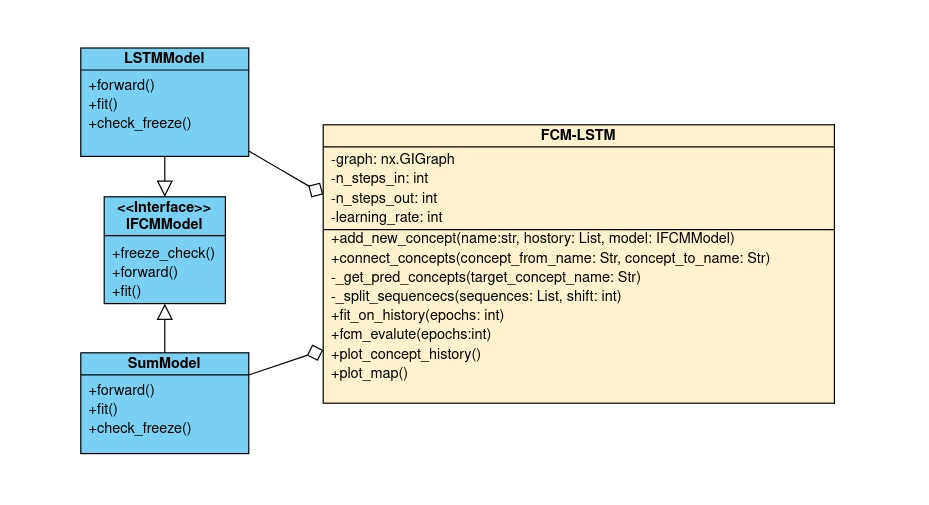
\includegraphics[height=7cm]{./img/class_diag.jpg}
	\caption{Диаграмма классов проектируемого модуля}
	\label{img:class_diag}
\end{figure}

\section{Проектирование структуры когнитивной карты для моделирования количества продаж}

Исследуемые данные представляют из себя несколько временных рядов
за 5 лет по количеству продаж в 3 разных магазинах по 3 разным категориям:

\begin{itemize}
	\item Еда
	\item Товары для дома
	\item Товары для хобби
\end{itemize}

Процесс покупки продуктов --- это социально-экономический процесс.
Количество продаж может зависеть от локальных или национальных праздников.
Продажи по конкретным товарам могут возрастать, если на эти товары есть скидки или акции.
Но так же стоит помнит, что в случае, если товар не завезли,
продажи такого товара будут нулевыми. Но это не значит, что этот товар никому не нужен.

В данной работе будет построена упрощенная модель карты для предсказания количества продаж.
Но влияние экзогенных параметров будет исследовано на других моделях.

Общее количества продаж складывается из сумм продаж
по в каждом магазине:

\begin{equation}\label{eq:sales_total_simple_model}
	STORE\_SALES\_{i} = \sum_{j=1}^{M} CATEGORY\_SALES_{i,j}
\end{equation}

\noindent A продажи в каждом магазине складываются из продаж
товаров каждой категории:

\begin{equation}\label{eq:store_sales_simple_model}
	STORE\_SALES\_{i} = \sum_{j=1}^{M} CATEGORY\_SALES_{i,j}
\end{equation}

Тогда когнитивная карта будет содержать следующие вершины:

\begin{itemize}
	\item $ total\_sales $ --- общее количество продаж
	\item $ store\_id\_TX\_1 $ --- количество продаж в первом магазине
	\item $ store\_id\_TX\_1\_cat\_id\_FOODS $ --- количество продаж в первом магазине в категории "еда"
	\item $ store\_id\_TX\_1\_cat\_id\_HOBBIES $ --- количество продаж в первом магазине в категории "товары для хобби"
	\item $ store\_id\_TX\_1\_cat\_id\_HOUSEHOLD $ --- количество продаж в первом магазине в категории "товары для дома"
	\item $ store\_id\_TX\_2 $ --- количество продаж во втором магазине
	\item $ store\_id\_TX\_2\_cat\_id\_FOODS $ --- количество продаж во втором магазине в категории "еда"
	\item $ store\_id\_TX\_2\_cat\_id\_HOBBIES $ --- количество продаж во втором магазине в категории "товары для хобби"
	\item $ store\_id\_TX\_2\_cat\_id\_HOUSEHOLD $ --- количество продаж во втором магазине в категории "товары для дома"
	\item $ store\_id\_TX\_3 $ --- количество продаж в третьем магазине
	\item $ store\_id\_TX\_3\_cat\_id\_FOODS $     --- количество продаж в третьем магазине в категории "еда"
	\item $ store\_id\_TX\_3\_cat\_id\_HOBBIES $   --- количество продаж в третьем магазине в категории "товары для хобби"
	\item $ store\_id\_TX\_3\_cat\_id\_HOUSEHOLD $ --- количество продаж в третьем магазине в категории "товары для дома"
\end{itemize}

Для моделирования продаж по каждой категории в конкретном магазине
будет использоваться LSTM.
Таким образом имея предсказания продаж для товаров каждой категории в каждом магазине
мы можем явно вычислить количество продаж в магазине целиком и в сумме для трех магазинов.
Для этого необходимо просуммировать результат предсказаний каждой категории
в каждом магазине --- $ CATEGORY\_SALES_{i,j} $.
Для этого при построении карты для значений концептов

\begin{itemize}
	\item $ total\_sales $
	\item $ store\_id\_TX\_1 $
	\item $ store\_id\_TX\_2 $
	\item $ store\_id\_TX\_3 $
\end{itemize}

\noindent будет использоваться простая модель для суммирования.
Особенность ее заключается в том, что модель LSTM в вершинах FCM-LSTM работает
с предыдущими историческими значениями концептов. А модель по суммированию должна работать
с уже предсказанными результатами модели LSTM.

Граф спроектированной карты представлен на рисунке \ref{img:fcm_lstm_map}.

\def\figurename{Рис}
\begin{figure}[t]
	\centering
	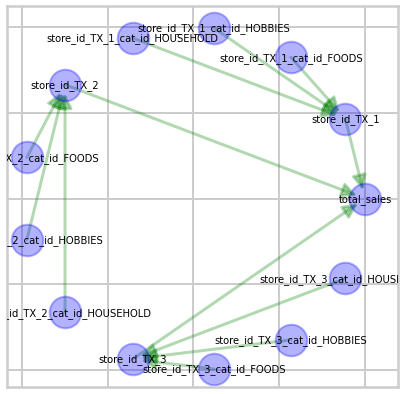
\includegraphics[width=0.5\columnwidth]{./img/fcm_lstm_map.png}
	\caption{Граф когнитивной карты для моделирования общего количества продаж с разбивкой по магазинам и категории товаров}
	\label{img:fcm_lstm_map}
\end{figure}

Все параметры в данной карте представляют из себя четкие числа.
Для исследуемого процесса нет возможности найти данные, которые
можно было бы использовать как нечеткие параметры.
Однако стоит заметить, что использование нечетких параметров
в разработанной системе все еще возможно:
четкие карты --- это частный случай нечетких.

\section{Выбор инструментальных средств}

В качестве языка программирования для проведения экспериментов и анализа данных
будет использоваться python. Это язык с динамической типизацией, но зато с
большим количеством хорошо протестированных и отлаженных фреймворков и библиотек для работы
с данными ($numpy$ \cite{oliphant2006guide}, $pandas$ \cite{reback2020pandas}), статистическим анализом ($statmodels$ \cite{seabold2010statsmodels})
и фреймфорками для построения нейросетей ($pytorch$ \cite{NEURIPS2019_9015}, $tensorflow$ \cite{tensorflow2015-whitepaper} ).

Для распараллеливания работы с данными и использовании аппаратных ускорений для умножений матриц
для реализации модуля подсистемы обработки данных и подсистемы для вычисления нечеткой карты
будет использоваться $pytorch$. Это фреймворк для работы с данными и созданию нейросетей.

Конкурентом $pytorch$ является $tensorflow$, но за счет того, что в $pytorch$ не статический
граф вычислений, а динамический, $pytorch$ предоставляет больше свободы, но и больше мест,
где можно ошибиться.

Недостатком python можно считать динамическую типизацию. Динамическая типизация не позволяет
найти многие ошибки на стадии компиляции. Многие ошибки можно обнаружить только во время
работы программы. Для того, чтобы бороться с этим недостатком, вместе с кодом нужно писать
автоматические тесты --- они позволяют быстро проверить работоспособность программы.

Для написания автоматических тестов был выбран фреймворк $ pytest $ \cite{pytestx.y}. В этом фреймворке
вводится понятие фикстур. Это помогает разделить тело теста (логику тести) и
подготовку данных для тестирования. Фикстуры позволяют сохранять тело
теста более чистым. Это позволяет быстро определить, в чем именно заключается ошибка.
Кроме того, благодаря возможности параметризации фикстур и теста, можно
запустить один и тот же тест с разными наборами данных.

Для работы с графами был выбран фреймворк $ networkx $ \cite{hagberg-2008-exploring}. Данный фреймворк
обладает удобным интерфейсом для построения и работы с графами и
позволяет визуально представить построенный граф.

Для разработки, отладки разрабатываемых модулей а так же для
анализа данных использовалась интерактивная среда вычислений Jupyter Notebook \cite{Kluyver:2016aa}.


\section{Выводы}

В данном разделе:

\begin{itemize}
	\item были рассмотрена архитектура системы непрерывной интеграции;
	\item выставлены функциональные требования к разрабатываемой модели;
	\item спроектирован интерфейс модуля;
	\item спроектирована архитектура когнитивной карты для моделирования количества продаж.
\end{itemize}

